\section{Modell des \spd-Systems}\label{sec:spdModell}


Die Modellierung des \spd-Systems orientiert sich zunächst an den Modellen der vergangenen Arbeiten. 
Diese bezogen sich auf die Herleitung von \cite{modpen}. 
Dabei gibt es die Variante \emph{Kraftsystem}, das als Eingang die Kraft annimmt, welche am Schlitten wirkt, sowie das vereinfachte \emph{Beschleunigungssystem}, das direkt die Beschleunigung des Schlittens als Eingang erhält.


%\begin{figure}[bp]
	%\centering
		%\includegraphics[width=0.7\textwidth]{Bilder/intro.pdf}
	%\caption{Idee des zentralen Reglerentwurfs}
	%\label{fig:intro}
%\end{figure}

\begin{figure}[h]
	\centering
		\begin{tikzpicture}[scale=1, auto, >=stealth',x=1cm,y=1cm]

	\def\pu{30}
	\def\lu{3}
	\def\su{2}
	
	\def\po{50}
	\def\lo{2.5}
	\def\so{1}

	\draw[thick] (-1,-0.5) |- (1,0.5) |- cycle;
	
	%\path (0,0) ++(\pu+90:\su) coordinate (su);
	%\path (0,0) ++(\pu+90:\lu) coordinate (lu);
	
	
	\begin{scope}[rotate=\pu]
		\draw[fill=white,thick] (1mm,0) -- (1mm, \lu) arc[start angle=0, end angle=180, radius=1mm] 
						-- (-1mm, 0) arc[start angle=180, end angle=360, radius=1mm];
		\draw[] (0,0) circle[radius=0.5mm];
		\draw[fill=black] (0, \su) circle[radius=0.5mm];
		
		\path (0, \su) coordinate (su);
		\path (0, \lu) coordinate (lu);
		
		\draw[very thin] (-1.5mm, 0) -- (-7.5mm, 0);
		\draw[very thin] (-1.5mm, \su) -- (-3.5mm, \su);
		\draw[white, <->] (-3mm, 0) -- (-3mm, \su); 
		\draw[very thin, <->] (-3mm, 0) -- node[pos=0.75,inner sep=0pt]{$s_1$} (-3mm, \su);

		\draw[very thin] (-1.5mm, \lu) -- (-7.5mm, \lu);
		\draw[white, <->] (-7mm, 0) -- (-7mm, \lu); 
		\draw[very thin, <->] (-7mm, 0) -- node[pos=0.75,inner sep=0pt]{$l_1$} (-7mm, \lu);
	\end{scope}
	
	\begin{scope}[rotate=\po,shift={(lu)}]
		\draw[fill=white,thick] (1mm,0) -- (1mm, \lo) arc[start angle=0, end angle=180, radius=1mm] 
						-- (-1mm, 0) arc[start angle=180, end angle=360, radius=1mm];
		\draw[] (0,0) circle[radius=0.5mm];
		\draw[fill=black] (0, \so) circle[radius=0.5mm];
		
		\path (0, \so) coordinate (so);
		\path (0, \lo) coordinate (lo);
		
		\draw[very thin] (-1.5mm, 0) -- ++(-2mm, 0);
		\draw[very thin] (-1.5mm, \so) -- ++(-2mm, 0);
		\draw[white, <->] (-3mm, 0) -- (-3mm, \so); 
		\draw[very thin, <->] (-3mm, 0) -- node[pos=0.5,inner sep=0pt]{$s_2$} (-3mm, \so);
	\end{scope}

	\draw[thick,white,->] (0,1.8) arc[start angle=90, end angle=90+\pu, radius=1.8cm];
	\draw[thin,->] (0,1.8) arc[start angle=90, end angle=90+\pu, radius=1.8cm];
	\node at (90+\pu/2:1.5cm) {$\varphi_1$};
	\draw[thin,dashed] (0,0) -- (0, 2);
	
	\draw[thick,white,->] (lu) ++(0,1.8) arc[start angle=90, end angle=90+\po, radius=1.8cm];
	\draw[thin,->] (lu) ++(0,1.8) arc[start angle=90, end angle=90+\po, radius=1.8cm];
	\path (lu) +(90+\po/2:1.5cm) node {$\varphi_2$};
	\draw[thin,dashed] (lu) -- ++(0, 2);


	\node[anchor=south east] at (1,-0.5) {$m_0$};
	
	\draw[very thin] (90+\pu:0.9*\lu) -- ++(8mm,3mm) node[anchor=west] {$m_1$, $J_1$};
	\draw[very thin] ($(lu)!0.9!(lo)$) -- ++(-8mm,-3mm) node[anchor=east] {$m_2$, $J_2$};
	
	
	\draw[thin] (-1.5,-1) -- ++(0,-0.5);
	\draw[thin,->] (-1.5,-1.25) -- node{$x_0$} (0,-1.25); 
	
	\draw[thin,->] (-3,0) -- ++(0.5,0) node[anchor=south, inner sep=1pt]{\tiny $x$};
	\draw[thin,->] (-3,0) -- ++(0,0.5) node[anchor=west, inner sep=1pt]{\tiny $y$};
	
\end{tikzpicture}

			\caption{\dpd}
	 \label{fig:koord}
\end{figure}

\subsection{Koordinaten}

Das System aus Schlitten und Doppelpendel hat 3 Freiheitsgrade, die mit den \emph{Minimal-\koor} 
\begin{align*}
	q_0 = x_0  \\
	q_1 = \varphi_1  \\
	q_2 = \varphi_2
\end{align*}
beschrieben werden. Die Koordinaten sind nach \figref{fig:koord} definiert.

Die Schwerpunktskoordinaten der Pendelstäbe ergeben sich zu
\begin{align*}
	\xe &= \xo - s_1 \sin{\phe}  \\
	\ye &=       s_1 \cos{\phe}  \\
	\xz &= \xo - l_1 \sin{\phe} - s_2 \sin{\phz}  \\
	\yz &=       l_1 \cos{\phe} + s_2 \cos{\phz}  \ .
\end{align*}


\subsection{Herleitung der Bewegungsgleichungen}\label{subsec:bwgl}

Um auf die \bwgl\ des Systems zu gelangen, wird in \cite{modpen} der \emph{Lagrange}-Formalismus verwendet. 
Dazu werden zunächst die kinetische und potentielle Energie des Gesamtsystems bestimmt sowie die nicht-konservativen Kräfte/Momente. 

Die kinetische Gesamtenergie ergibt sich zu
\begin{align}
	T = \einhalb m_0 \, \xop^2 + \einhalb m_1 (\xep^2+\yep^2) + \einhalb m_2 (\xzp^2+\yzp^2) + \einhalb J_1 \, \phep^2 + \einhalb J_2 \, \phzp^2
\end{align}
und die potentielle Energie beträgt
\begin{align}
	U = m_1\, g\, \ye + m_2\, g\, \yz  \ .
\end{align}

Die nicht-konservativen Kräfte/Momente setzen sich aus der Antriebskraft $F$ am Schlitten (in~$\xo$-Richtung) und den Reibungs-Kräften/Momenten zusammen und lauten
\begin{subequations} \begin{align}
	Q_0^* &= F + \Fd + \Fc  \\
	Q_1^* &= \Mde + \Mce - \Mdz - \Mcz  \\
	Q_2^* &= \Mdz + \Mcz
\end{align} \end{subequations} 
mit den viskosen Dämpfungen
\begin{subequations} \label{eq:visd} \begin{align}
	\Fd  &= -d_0 \xop  \\
	\Mde &= -d_1 \phep  \\
	\Mdz &= -d_2 \left(\phzp-\phep\right)  
\end{align} \end{subequations} 
sowie den \crb en $\Fc$, $\Mce$ und $\Mcz$, welche in \secref{sec:crb} genauer betrachtet werden.

Mit dem Formalismus ergeben sich die 3 \emph{gekoppelten} Bewegungsgleichungen für die Minimal-\koor. 
Um nach den zweiten Ableitungen aufzulösen, muss allerdings noch das \gls\ gelöst werden.

Damit ergeben sich die \bwgl\
\begin{align*}
	\xopp  &= f_{\xo}(\dots)  \\
	\phepp &= f_{\phe}(\dots)  \\
	\phzpp &= f_{\phz}(\dots)
\end{align*}
als Funktion der Minimal-\koor, der Systemparameter und des Eingangs.

Die Berechnung der Ableitungen und das Lösen des \gls s geschah bisher händisch, was im Allgemeinen fehleranfällig ist. 
In dieser Arbeit werden die \bwgl\ mithilfe der \emph{symbolischen Toolbox} von \ml\ gelöst. 
Die für den \emph{Lagrange}-Formalismus benötigten Ableitungen werden symbolisch berechnet und das \gls\ mit dem symbolischen Solver gelöst und vereinfacht. 
Diese Vorgehensweise ist nicht nur weniger fehleranfällig, dadurch lässt sich das System auch sehr flexibel modifizieren.


\subsection{\zrm}\label{subsec:zrm}

Um das \spds\ als \zrm\ (mit ausschließlich ersten Ableitungen) darzustellen, wird folgender Zustandsvektor definiert:
\begin{align}
	\vex = \begin{bmatrix}
		x_1 \\	x_2 \\	x_3 \\	x_4 \\	x_5 \\	x_6 \\	
	\end{bmatrix} = \begin{bmatrix}
		\xo \\ \xop \\ \phe \\ \phep \\ \phz \\ \phzp
	\end{bmatrix}
	\label{eq:vex}
\end{align}
Mit den \bwgl\ ergibt sich für das \krs\ (Eingangsgröße $u=F$) das folgende nichtlineare, eingangsaffine \zrm:
\begin{align}
	\vexp &= \ve{f}(\vex,u)  \\
		&= \ve{a}(\vex) + \ve{b}(\vex) \cdot F  
		\label{eq:zrm} 
		\\\vspace{100cm}
	\ddt \begin{bmatrix}
		\xo \\ \xop \\ \phe \\ \phep \\ \phz \\ \phzp
	\end{bmatrix} &= \begin{bmatrix}
		f_1(\vex,u) \\ f_2(\vex,u) \\  f_3(\vex,u) \\  f_4(\vex,u) \\  f_5(\vex,u) \\  f_6(\vex,u)
	\end{bmatrix}= \begin{bmatrix}
		\xop \\ a_2(\vex) \\ \phep \\  a_4(\vex) \\ \phzp \\  a_6(\vex)
	\end{bmatrix} + \begin{bmatrix}
		0 \\ b_2(\vex) \\ 0 \\  b_4(\vex) \\ 0 \\  b_6(\vex)
	\end{bmatrix} \cdot F
	\label{eq:zrmF}
\end{align}

Beim Beschleunigungssystem gilt für den Eingang $u=\xopp=a$, womit die Schlittenbeschleunigung direkt vorgegeben und die Dynamik des Schlittens umgangen wird. 
Damit wird die erste der drei gekoppelten Bewegungsgleichungen ersetzt. 
Das geänderte \gls\ muss wieder gelöst werden und für das \zrm\ folgt:
\begin{align}
	\ddt \begin{bmatrix}
		\xo \\ \xop \\ \phe \\ \phep \\ \phz \\ \phzp
	\end{bmatrix} &= \begin{bmatrix}
		\xop \\ 0 \\ \phep \\  a_4(\vex) \\ \phzp \\  a_6(\vex)
	\end{bmatrix} + \begin{bmatrix}
		0 \\ 1 \\ 0 \\  b_4(\vex) \\ 0 \\  b_6(\vex)
	\end{bmatrix} \cdot a
	\label{eq:zrmA}
\end{align}

\tabref{tab:abh} gibt Aufschluss über die Abhängigkeiten von Zuständen und \syp n. 
Grau hinterlegte Variablen sind nur im Kraftmodell vorhanden. 
Der Zustand \xo\ hat keinen Einfluss auf die Systemdynamik.
\begin{table}[h]
	\centering
	\caption{Abhängigkeiten von Zuständen und Parametern}
		\begin{tabular}[t]{ll}
		\toprule
			Zustände	&	\textcolor{grey}{\xop}, \phe, \phep, \phz, \phzp	\\
			Trägheitsparameter	&	\textcolor{grey}{$m_0$}, $m_1$, $m_2$, $J_1$, $J_2$ \\
			Geometrieparameter	&	$l_1$, $s_1$, $s_2$	\\
			Reibungsparameter	&	\textcolor{grey}{$d_0$}, $d_1$, $d_2$, \textcolor{grey}{\Fco}, \Mceo, \Mczo, \textcolor{grey}{\xopth}, \pheth, \phzth	\\
			Umgebungskonstanten & $g$	\\
			\bottomrule
		\end{tabular}
	\label{tab:abh}
\end{table}


Am Versuchsstand können die Schlittenposition und beide Pendelwinkel über Sensoren gemessen werden. Daher ergibt sich für den Ausgang beider Systeme:
\begin{align}
	\ve{y} = \ve{h}(\vex)
	= \mat{C} \vex
	= \begin{bmatrix}
		1 & 0 & 0 & 0 & 0 & 0 \\
		0 & 0 & 1 & 0 & 0 & 0 \\
		0 & 0 & 0 & 0 & 1 & 0 
	\end{bmatrix} \vex
	= \begin{bmatrix}
		\xo \\ \phe \\ \phz
	\end{bmatrix}  \ .
	\label{eq:hx}
\end{align}
Es handelt sich demnach um ein \emph{SIMO-System} (single input multiple output). 


\subsection{\crb}\label{sec:crb}

Neben der einfach zu beschreibenden viskosen Dämpfung \eqref{eq:visd} gibt es in der Realität komplexere Arten von Reibung, die die Systembeschreibung erschweren. 
Eine Übersicht zu verschiedenen Reibungsmodellen ist in \cite{ribeiro} gegeben.

Da die \crb\ sowohl des Schlittens als auch der Pendelstäbe einen wesentlichen Einfluss zu haben scheint, darf diese nicht vernachlässigt werden. 
In den bisherigen Modellierungen wurde höchstens die \crb\ des Schlittens berücksichtigt. 
Bei der Neukonstruktion ist jedoch in den Gelenken eine höhere \crb\ vorhanden \siehe{\secref{subsec:spdparams}}, weswegen diese ebenfalls modelliert wird.
Die eigentlich vorhandene Haftreibung wird nicht modelliert.

Die Formel der Gleitreibung lautet eigentlich 
	\[
	\Fc = \Fco  \cdot  \sign{\xop} \ ,
\]
allerdings führt diese Implementierung aufgrund der $\operatorname{signum}$-Funktion \siehe{\figref{fig:signs}} zu Komplikationen in der Simulation.
In der Nähe des Vorzeichenwechsels ist die Funktion unendlich steil, was bei Nulldurchgängen in der Simulation problematisch ist, weil die Schrittweite dadurch sehr klein werden muss.
Zwar kann man in \sm\ die Option \qq{Zero Crossing Detection} abschalten, es kommt dann allerdings meistens zu einem \qq{Rattern}. 
\cite{modsim}


\begin{figure}[b]
	\centering
	\subfloat[\sign{x}]{ 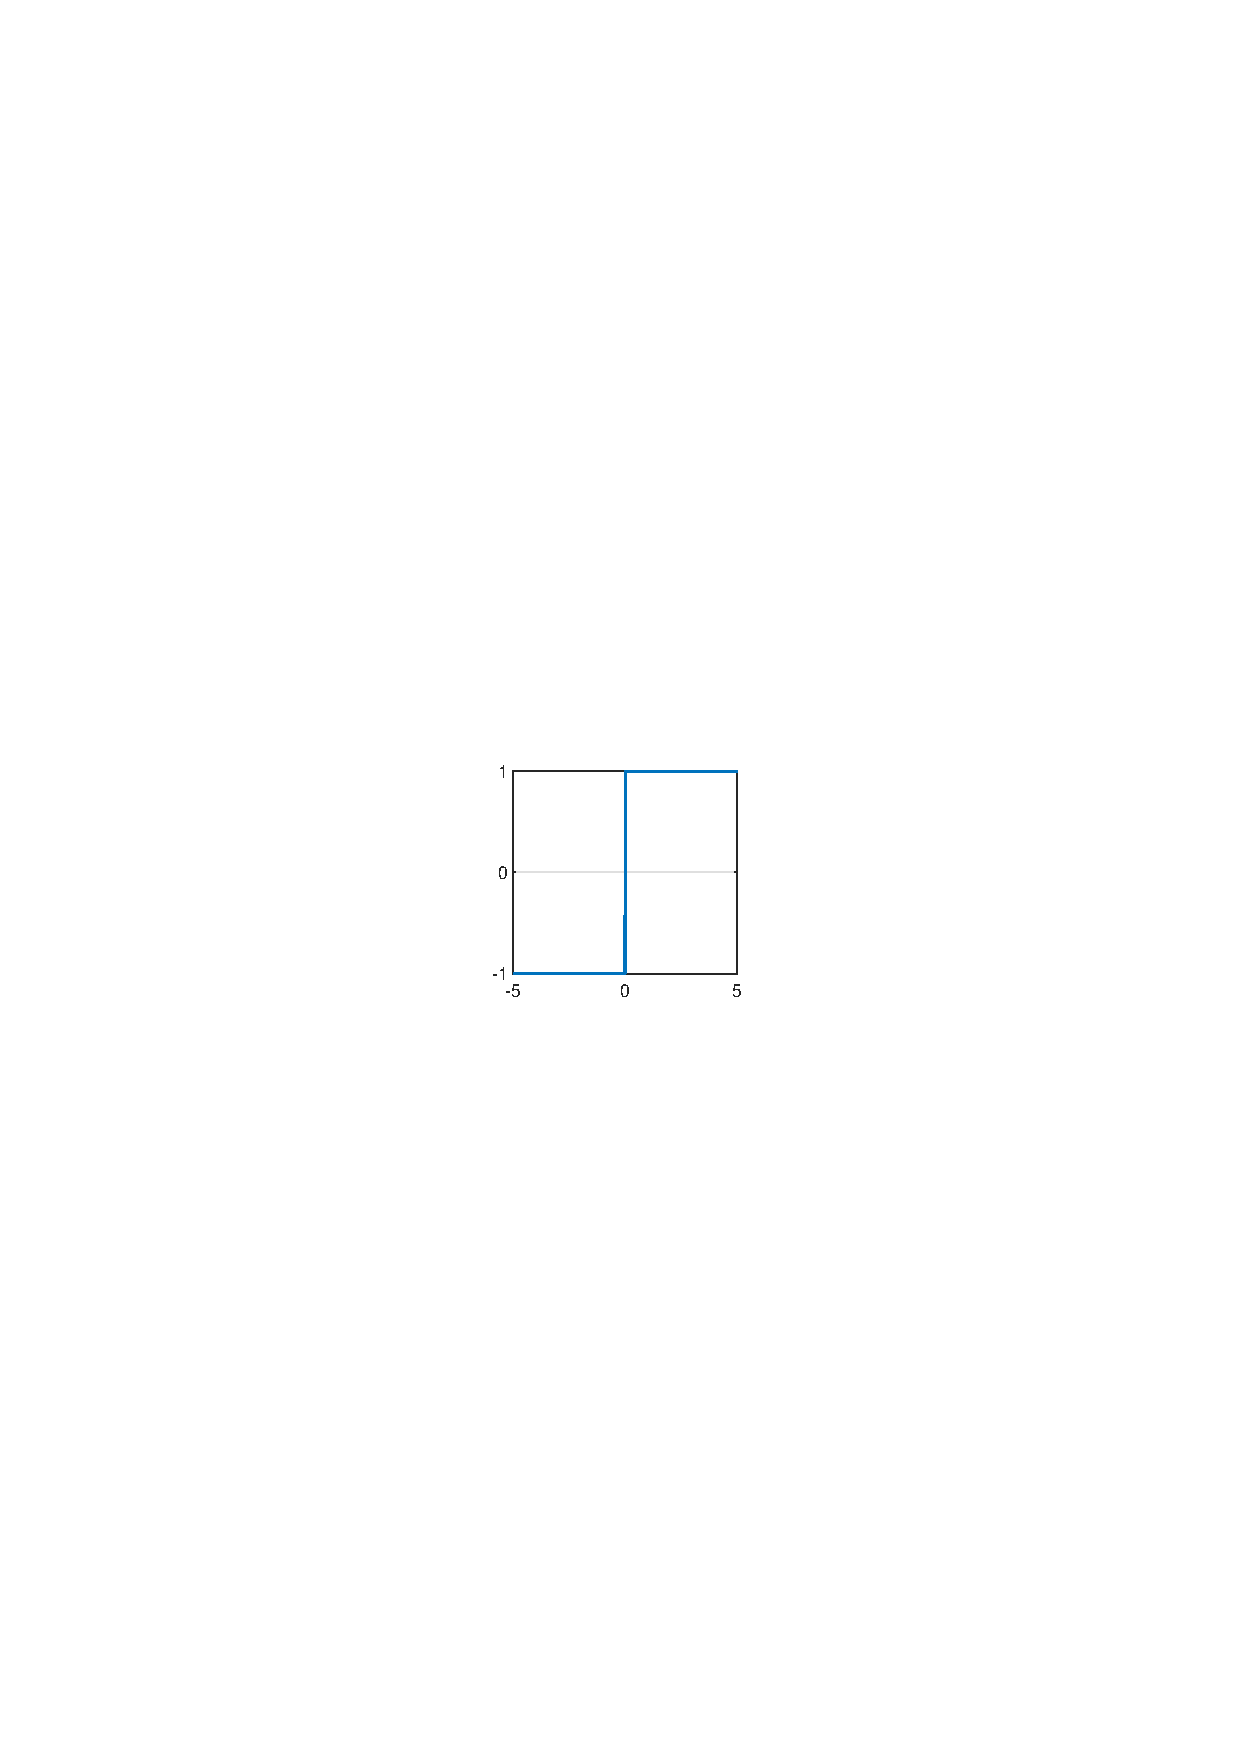
\includegraphics[scale=1]{Bilder/sign/sign.pdf}	 \label{fig:signs}}
	%\hfil
	\subfloat[$\frac{2}{\pi} \arctan{(x)}$]{	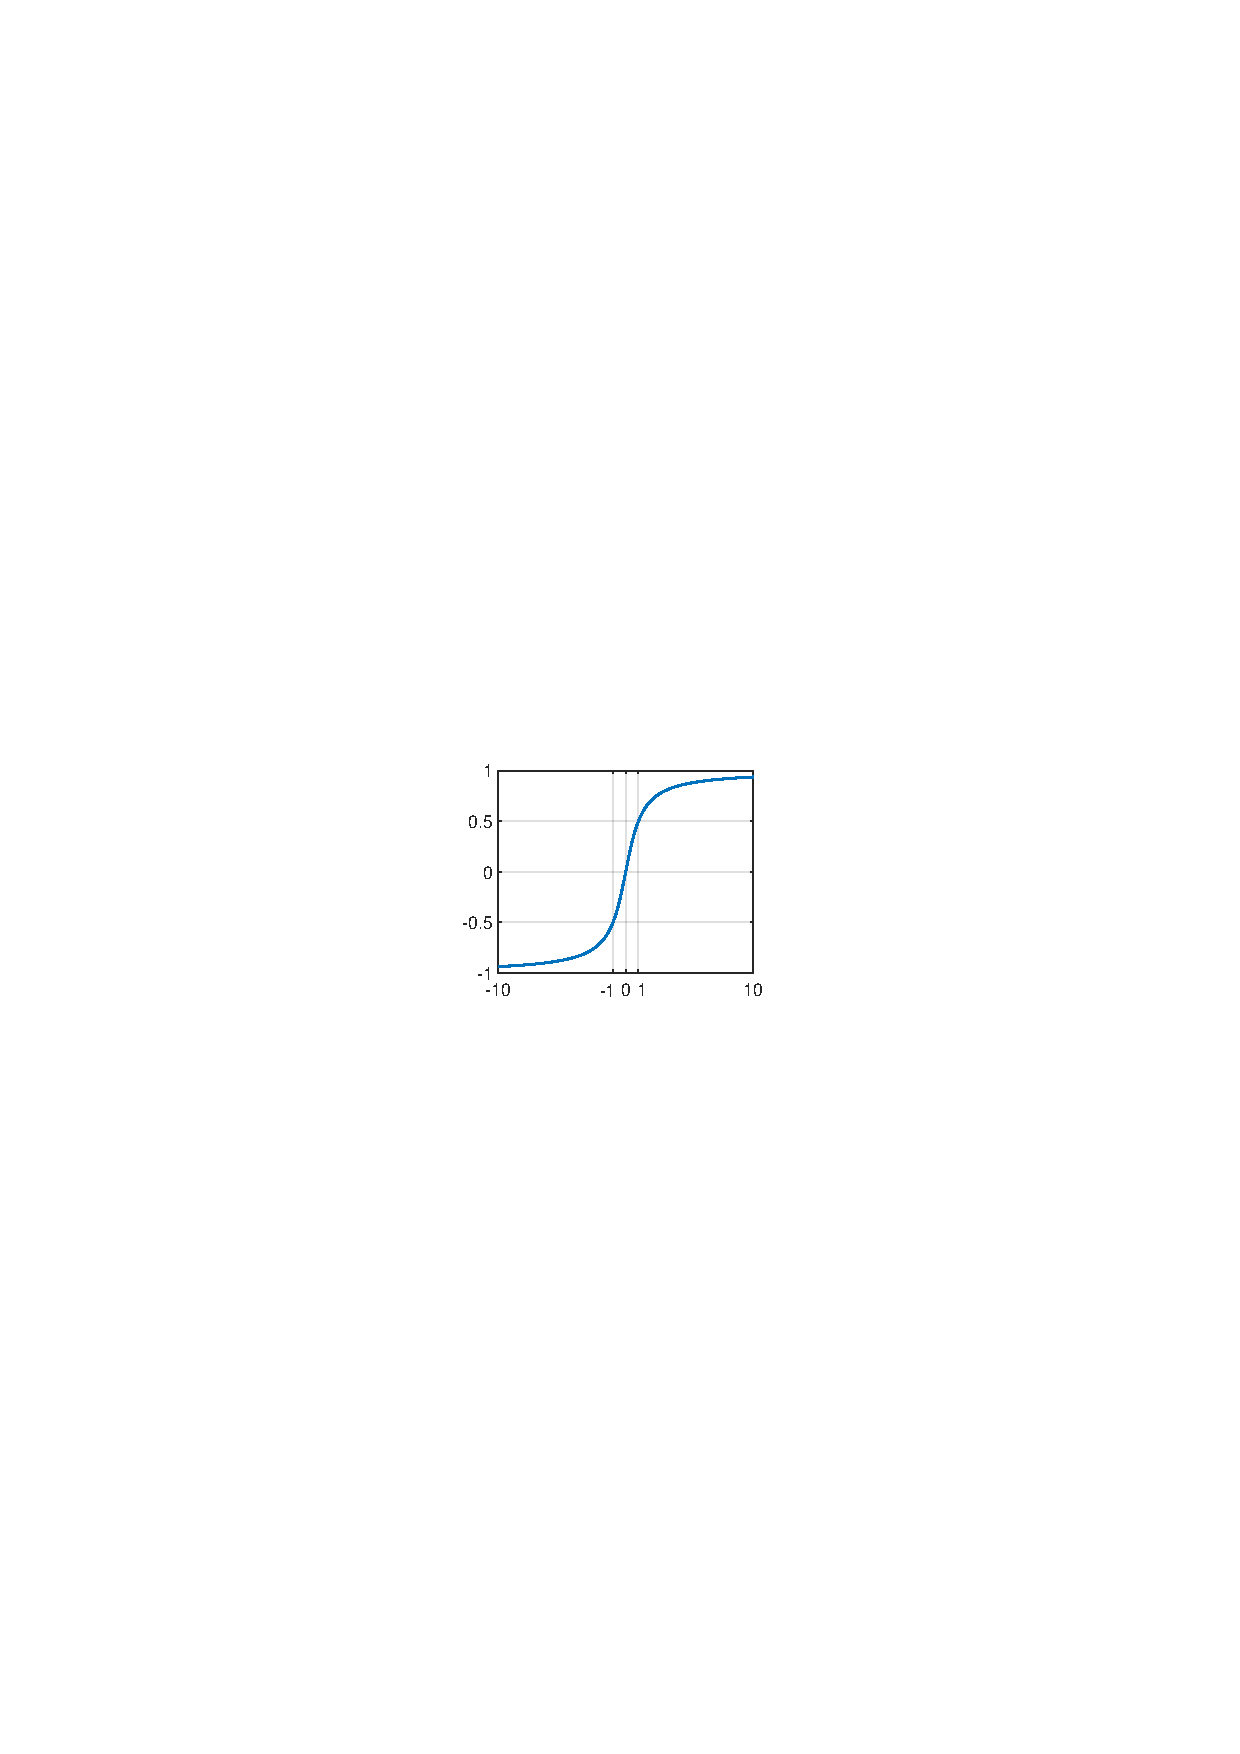
\includegraphics[scale=1]{Bilder/sign/2-pi-atan.pdf}	 \label{fig:atan}}
	%\hfil
	\subfloat[$\tanh{(x)}$]{ 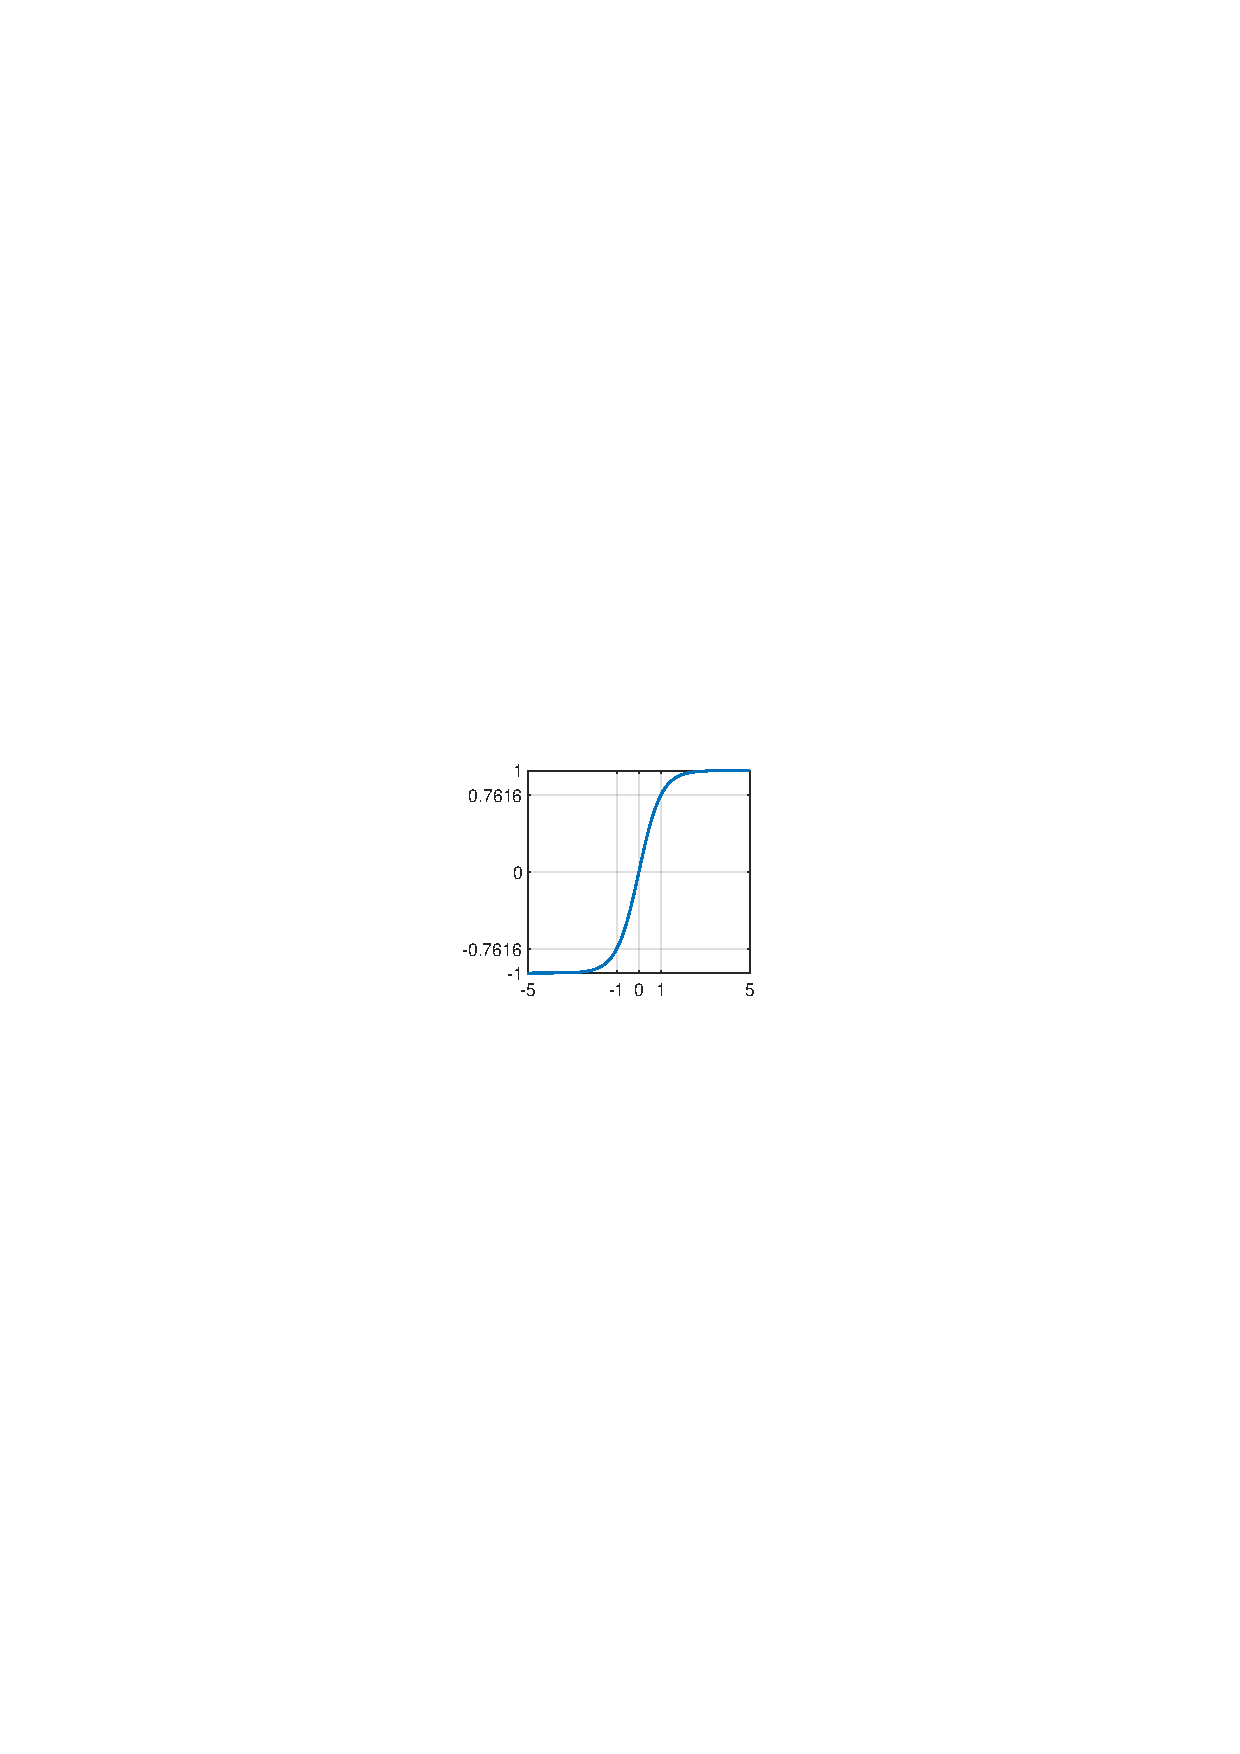
\includegraphics[scale=1]{Bilder/sign/tanh.pdf} \label{fig:tanh}} 
	\caption{Annäherung \mrm{signum}-Funktion -- Vergleich}
	\label{fig:sign}
\end{figure}

In \cite{chang} und \cite{kisner} wurde der Verlauf der $\operatorname{signum}$-Funktion bei sehr niedrigen Geschwindigkeiten mit der $\arctan$ Funktion angenähert \siehe{\figref{fig:atan}}.
	\[
		\Fc=\Fco \cdot \frac{2}{\pi} \arctan \left(\frac{\xop}{150}\right)
\]
Die Funktion nähert sich jedoch nur sehr langsam dem Endwert an.
In dieser Arbeit wird daher die $\tanh$ Funktion verwendet, welche deutlich früher den Endwert annimmt \siehe{\figref{fig:tanh}}.
%
\begin{subequations} \begin{align}
	\Fc  &= -\Fco  \cdot \tanh{\left(\frac{\xop}{\xopth}\right)}  \\
	\Mce &= -\Mceo \cdot \tanh{\left(\frac{\phep}{\pheth}\right)}  \\
	\Mcz &= -\Mczo \cdot \tanh{\left(\frac{\phzp-\phep}{\phzth}\right)}
 \end{align} \end{subequations}
Dabei ist $\xopth$ gerade die Geschwindigkeit, bei der $\tanh(1)=0.7616$ von $\Fco$ erreicht ist.



\subsection{Ruhelagen}\label{sec:aps}

Die Ruhelagen \bzw \ap e eines nichtlinearen Systems ergeben sich aus
	\[
	\vexp_R = \ve{f}(\vex_R,u_R) = \ve{0}  \ .
\]
Für das \spds\ gibt es aufgrund der Periodizität von Sinus und Kosinus theoretisch unendlich viele Ruhelagen. 
Es werden daher die folgenden 4 prinzipiell unterschiedlichen betrachtet:
\begin{table}[h]
	\centering
	\caption{Die 4 Ruhelagen}
		\begin{tabular}{ccccccccc}
		\toprule
			\ap  & $u$ & \xo & \xop & \phe & \phep & \phz & \phzp & Stabilität  \\
			\midrule
			1	&	0 &	\xor	&	0	&	\pii	&	0	&	\pii	&	0	& stabil  \\
			2	&	0 &	\xor	&	0	&	\pii	&	0	&	0			&	0	& instabil  \\
			3	&	0 &	\xor	&	0	&	0			&	0	&	\pii	&	0	& instabil  \\
			4	&	0 &	\xor	&	0	&	0			&	0	&	0			&	0	& instabil  \\
			\bottomrule
		\end{tabular}
	\label{tab:aps}
\end{table}

Die Schlittenposition \xo\ ist dabei beliebig, da der Schlitten an jeder Position eine Ruhelage annehmen kann.
Die Reihenfolge der \ap e entspricht den Pendelpositionen \qq{von unten nach oben}.


\subsection{Beschränkungen}\label{sec:schlbes}

Die Länge der Schlittenführung ist am realen Versuchsstand endlich, weswegen die Schlittenposition begrenzt ist.
Es gilt für die Position des Schlittenmittelpunktes:
	\[ 
	 \valunit{-0,8}{m} \leq \xo \leq \valunit{0,8}{m}
\]